\chapter{Blockchain: il funzionamento e\\ i concetti principali}
\label{ch:blockchain}
% --- Inizio sezione 2 ---

Seguendo l’impostazione del lavoro presentata nell’introduzione è possibile individuare una prima nozione ricorrente, quella di “registro distribuito”. Negli ultimi anni l’estensione di Internet ha permesso di muovere i registri e generalmente parlando dati, da un supporto fisico a un supporto digitale attraverso l’utilizzo delle basi di dati sparse in tutto il mondo. Tuttavia, la struttura attuale delle basi di dati, e per certi aspetti l’architettura odierna di Internet, presenta dei problemi e svantaggi che con l’andare del tempo non si è riusciti a risolvere in maniera definitiva. Basti pensare ai problemi relativi alla sicurezza, affidabilità e centralizzazione delle risorse memorizzate in rete.

Problematiche che, nella maggior parte dei contesti, possono essere ricondotte alla commercializzazione e centralizzazione delle risorse. Il punto chiave è che Internet allo stato attuale, Internet delle informazioni, si avvale di intermediari. Aziende come Google, Microsoft, Amazon e Facebook controllano una quantità enorme di informazioni e attività dei propri utenti. Un esempio del fenomeno può essere indotto dall’offerta di servizi di cloud computing (*aaS, anything as a service). Senza dubbio il vantaggio di questi servizi, è che permettono agli utenti di usare risorse senza dover investire in un’infrastruttura propria e che sono offerti ad un costo relativamente basso. Si tratta pur sempre di intermediari verso quali è necessaria la fiducia che con il passare del tempo le corporazioni non sempre hanno dimostrato di gestire in maniera soddisfacente. Sono sorte preoccupazioni, circa questioni importanti come la sicurezza, la censura e l'affidabilità di questi sistemi. Più in generale, i sintomi negativi della centralizzazione sono evidenti quando si parla dei problemi relativi alla privacy e uso inopportuno di dati privati, temi che ultimamente emergono di frequente. Ecco che avere opzioni, alternative in più a quelle già esistenti, può essere importante al fine di mitigare i rischi che possono essere causati da una situazione di monopolio e concentrazione del potere nelle mani dei pochi.

La blockchain è un paradigma oppure semplificando, una tecnologia che potrebbe portare a una nuova evoluzione, un potenziale passaggio da un Internet delle informazioni all’Internet dei valori. Grazie all’uso della crittografia, il sistema di firme digitali, il networking peer-to-peer (P2P) e algoritmi di consenso, gli utenti possono effettuare transazioni che verranno mantenute in registri distribuiti, immutabili e permanenti senza bisogno di intermediari. In questo capitolo verranno descritti i concetti che formano l’insieme delle componenti di base delle blockchain.


\section{La struttura delle blockchain}

I concetti relativi alla struttura possono essere derivati dalla sua prima implementazione. Nel 2008 nasce Bitcoin, la prima applicazione su larga scala della tecnologia di seguito denominata blockchain. Fondata da Satoshi Nakamoto (autore o gruppo di autori anonimo), aveva come finalità la creazione di un sistema monetario digitale\footfullcite{Nakamoto_bitcoin:a}. Il sistema utilizza un registro pubblico, distribuito su tutti i nodi, contenente tutte le transazioni ordinate e valide, eseguite al suo interno fin dall’inizio della creazione del sistema stesso. Il concetto di sistema monetario digitale fu descritto già nel 1998 da Nick Szabo\footfullcite{SzaboDigCurr}, il quale aveva coniato il termine di certificati digitali al portatore (digital bearer certitifcate). Ancora prima, nel 1991, nell’articolo “How to Time-Stamp a Digital Document” di Stuart Haber e W. Scott Stornetta\footfullcite{Haber91howto} furono descritte quelle che sono le basi teoriche di un sistema decentralizzato. Questi documenti, rappresentano una fonte rilevante di approfondimento e sono importanti in quanto contengono l’espressione di concetti giudicati utili per la comunità ai fini di migliorare i sistemi digitali esistenti. Furono alla base della successiva ricerca sulla tecnologia, che ha condotto, a partire da Bitcoin, alla possibilità della sua implementazione concreta.

Al momento, esistono oppure sono in via di sviluppo molte applicazioni e sistemi che utilizzano le blockchain, spesso la loro struttura costituisce un’estensione o un adattamento più sofisticato dei concetti iniziali a seconda delle funzionalità offerte. Questa è la motivazione per cui saranno presentati principalmente i concetti universali anche in funzione degli obiettivi finali per fornire un collegamento alle loro implementazioni e infine al caso concreto dell’archivio digitale.


\subsection{Distribuzione e decentralizzazione}

Prima di passare ai dettagli strutturali delle catene dei blocchi, è importante distinguere tra due nozioni, quella di \emph{sistema distribuito} e \emph{decentralizzato}. Spesso, quando si parla di blockchain, i due termini sono usati come sinonimi. 

In realtà, dalle considerazioni precedenti è emerso che le blockchain implementano la tecnologia dei registri distribuiti collocando quest’ultima ad un livello di astrazione superiore. La DLT consiste nella condivisione di registri oppure, detto in un altro modo, base di dati a tutti i partecipanti del sistema. In questo caso, i sistemi in questione sono le blockchain che a loro volta vengono gestite da regole precise incapsulate nei sistemi di consenso (un argomento che verrà affrontato in dettaglio nel paragrafo 2.2). A questo punto, è sufficiente dire che grazie a questi sistemi di consenso, ogni nodo partecipante al sistema possiede una copia del registro e può interagire con esso effettuando modifiche che successivamente vengono aggregate con quelle di altri partecipanti. L’obiettivo è quello di mantenere una versione condivisa e sincronizzata del registro a tutti i partecipanti del sistema, in funzione delle regole di consenso della rete blockchain. Riassumendo, si ha una completa distribuzione quando tutti i partecipanti sono in possesso di uno stesso registro.

Per quanto riguarda la nozione di decentralizzazione, un approfondimento rilevante sulla questione è fornito in un articolo di Vitalik Buterin, uno dei fondatori del progetto Ethereum\footfullcite{Ethereum}. La sua idea è basata sulla suddivisione di un sistema e la sua centralizzazione o decentralizzazione lungo tre assi: quelli dell’architettura, della politica e della logica.
\\
\begin{figure}[H]
\centering
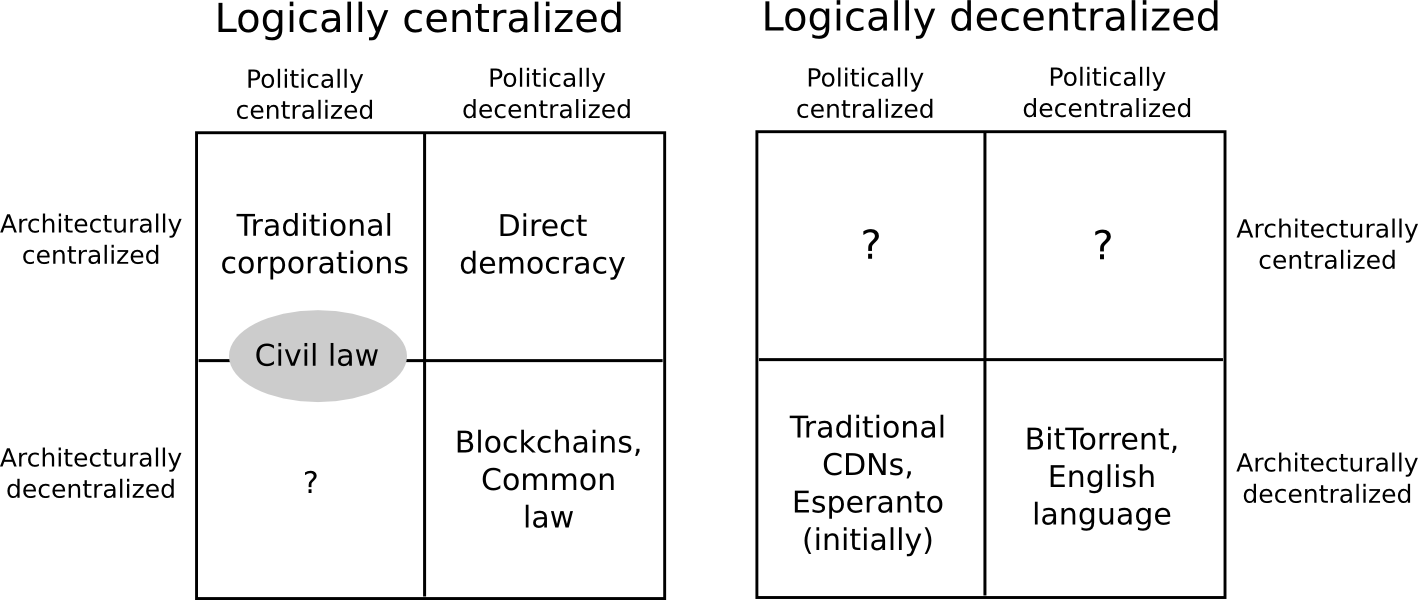
\includegraphics[width=1\textwidth]{immagini/meaning_decentralization.png}
\caption{Gli assi della decentralizzazione}
\label{fig:mesh1}

\end{figure}

Secondo l’autore, come illustrato nella figura 2.1, le blockchain sono architetturalmente e politicamente decentralizzate (nessuno esegue un controllo diretto su di esse e non c’è un punto centrale di guasto) ma logicamente centralizzate in quanto sono soggette a un preciso stato condiviso al momento dell'esecuzione del sistema che si comporta come un singolo computer\footfullcite{vitalButerinDecent}. Quest’ultimo aspetto, di nuovo, è fortemente legato ai protocolli di consenso che dipendono principalmente dalle varie tipologie di blockchain (un aspetto discusso nel paragrafo 2.4). La decentralizzazione riguarda maggiormente l’aspetto dei permessi dei partecipanti e governance sulla rete. La suddivisione descritta è valida per blockchain pubbliche (permissionless) sulle quali si concentra questa tesi, in cui tutti i partecipanti hanno pari diritti di agire e modificare il registro condiviso. Per quanto riguarda la tipologia delle blockchain con permessi (permissioned) la questione va riesaminata caso per caso a seconda dell’implementazione concreta. 

Uno tra tanti esempi di quest’ultima tipologia è Ripple\footfullcite{rippleMain}, blockchain per trasferimento di fondi che nel suo sistema di validazione si avvale di un certo numero di attori imposti a priori perché ritenuti fidati dall'azienda. Questa politica comporta dei vantaggi dal punto di vista della scalabilità e velocità di funzionamento a discapito della decentralizzazione dovuto alle forme di mediazione centralizzata. Attualmente, in questo specifico caso, con l’evoluzione della tecnologia blockchain questa strategia\footfullcite{rippleStrategy} viene rivista a favore di una maggiore decentralizzazione. Gli aspetti pro e contro l’adozione di sistemi più o meno decentralizzati sono discussi nel paragrafo (2.3.3).

Finalmente, distinte queste due nozioni è possibile arrivare alla seguente conclusione: il paradigma blockchain è distribuito (i partecipanti sono in possesso del registro replicato) mentre a livello inferiore, di implementazioni possono essere più o meno decentralizzate (o centralizzate) a seconda degli obiettivi e funzionalità che intendono raggiungere.

\subsection{Transazioni e concatenazione di blocchi}

Le blockchain utilizzano, letteralmente, una struttura pensata come una catena di blocchi. Ciascun blocco contiene al suo interno una lista di transazioni immutabili a loro volta contrassegnate da delle proprietà. Nelle attuali implementazioni le proprietà fondamentali sono: l’indirizzo mittente (input) e destinatario (output), l’ammontare di valuta o token contenuto nella transazione e la marcatura temporale (timestamp).

In una rete di consenso decentralizzato vengono man mano inseriti dei blocchi contenenti al loro interno un certo numero di transazioni. A livello universale, di rete, questa catena viene gestita dagli algoritmi di consenso come ad esempio: Proof of Work e Proof of Stake (descritti nel paragrafo 2.1.4) appendendo i blocchi giudicati validi dopo l'ultimo blocco valido della catena in modo da creare un registro di operazioni ordinato cronologicamente. Una volta stabilita la legittimità di un blocco e la sua appartenenza alla catena valida più lunga, l’intera struttura viene aggiornata propagando i nuovi elementi a tutti i partecipanti del sistema. Lo stato del registro a questo punto, non è più soggetto a modifiche, diventa permanente e immutabile. Successivamente, il procedimento riparte ricorsivamente, come descritto, ampliando la catena con le nuove operazioni.

Il primo blocco\footfullcite{genesisBitc} \smallskip \footfullcite{genesisEth} (hardcoded), originario di tutta la catena è chiamato \emph{genesi}. È un blocco speciale perché non è preceduto da altri blocchi, in esso vengono programmate le proprietà dei blocchi futuri. Le specifiche cambiano a seconda dell’implementazione. Generalmente, si tende a definire proprietà come la grandezza del blocco, la difficoltà di appendere nuovi blocchi e la ricompensa per la creazione (validazione) di nuovi blocchi nel sistema. 
Seguendo questo ragionamento, il seguente è un esempio valido di un blocco generico che eredita le sue proprietà dal blocco genesi.
Di seguito, insieme alle spiegazioni di alcuni concetti si forniscono pezzi di codice (code snippets) per illustrare la relativa struttura semplificata (il codice rispetta la sintassi Javascript ECMAScript 2015\footfullcite{jsDocs}). 
\\

\begin{lstlisting}[caption={Esempio di struttura di un blocco},language=JavaScript]
class block {
    constructor(timestamp, transactions, prevHash ='') {
        this.timestamp = timestamp;
        this.transactions = transactions;
        this.prevHash = prevHash;
        this.hash = this.calculateHash();
        this.nonce = 0;
    }
\end{lstlisting}

Ancora una volta, tra le proprietà importanti per il protocollo, si possono distinguere: la marcatura temporale che corrisponde alla data di creazione del blocco, la lista di transazioni incluse nel blocco, e la connessione tra i blocchi ovvero il "legame" calcolato tramite la funzione hash tra il blocco successivo e precedente.

Combinando insieme i blocchi si otterrà la seguente panoramica della struttura:

\begin{figure}[H]
\centering
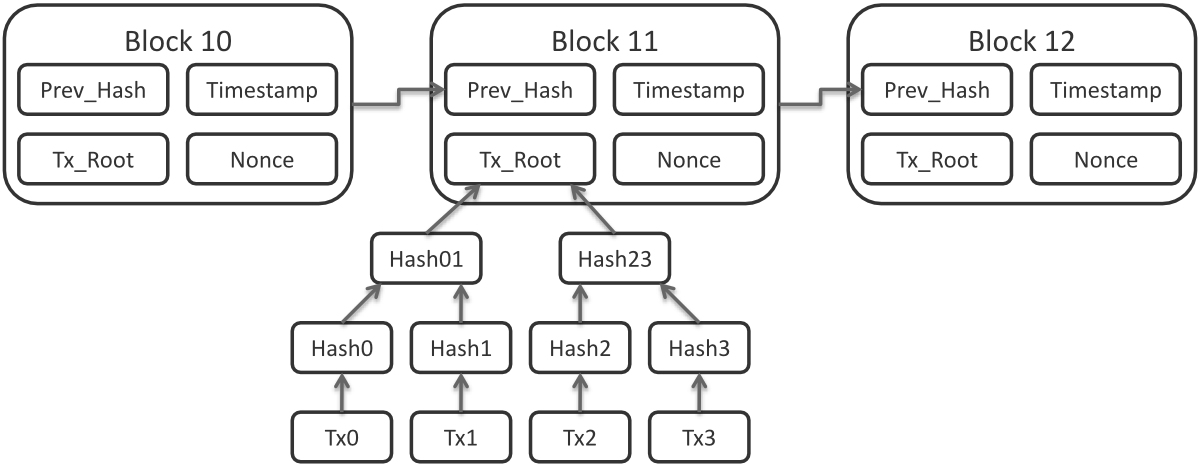
\includegraphics[width=1\textwidth]{immagini/bitcoinblocks.png}
\caption{Struttura semplificata di una catena di blocchi}
\label{fig:mesh2}

\end{figure}

Tenendo in mente che l'impostazione di un blocco può contenere un numero di proprietà variabile (a seconda dell'implementazione), è possibile generalizzare una struttura come quella illustrata nella figura 2.2. Nelle sezioni successive saranno analizzati gli elementi costituenti dei blocchi e le procedure che ne determinano il funzionamento.

\subsection{Funzioni di hash}

Ogni blocco è legato al blocco precedente tramite una funzione hash calcolata in base alle proprietà del blocco. Una funzione hash è una funzione matematica unidirezionale che accetta un input di lunghezza arbitraria e ne produce un output di lunghezza prefissata.

È una delle componenti base di una struttura formata da sequenze di blocchi che a sua volta è paragonabile alla struttura di una lista concatenata (linked list) tramite puntatori. In entrambi i casi la struttura permette di identificare in maniera univoca la relazione precedente e successivo che intercorre tra due blocchi. Data la definizione della funzione hash il cui risultato è contenuto tra le proprietà di ciascun blocco, è possibile formalizzare la seguente relazione:
\\

\begin{math} 
\forall\; n,\ \ \exists\; n - 1 \ \ |  \ \ PrevHash(n) = Hash(n-1),\; \forall\; n \neq genesi
\\
\end{math}

Per ogni blocco \begin{math} n \end{math} valido (ad eccezione del primo blocco della catena, genesi, dove la proprietà prevHash sarà uguale a 0) esiste un blocco \begin{math} n-1 \end{math} tale che, la funzione hash di \begin{math} n \end{math} è calcolata in base ai dati contenuti nel blocco precedente (\begin{math} n-1 \end{math}) con la risultante proprietà \begin{math} PrevHash(n) \end{math} equivalente ad un puntatore hash al blocco precedente. 
Il risultato del confronto precedente è che invece di un semplice indirizzo che punta al prossimo elemento della lista concatenata, nelle sequenze di blocchi si crea una funzione hash formata a partire dalle proprietà (dati) del blocco precedente.

Senza entrare troppo in dettaglio, questo implica un insieme di proprietà "grande" sulle quali vengono calcolate le funzioni hash con la caratteristica che anche una minima variazione di ciascun componente del dominio della funzione molto probabilmente farà cambiare radicalmente il risultato calcolato.

Nel seguente esempio si calcola la funzione hash applicando l'algoritmo SHA256 (Secure Hashing Algorithm)\footfullcite{sha2Wiki}, utilizzata nelle blockchain (per esempio Bitcoin) per due input apparentemente simili: 
\\

\begin{lstlisting}
//Input 1: ciao Tizio
>> SHA256("ciao Tizio")
//Output 1: 
>> 875647588afa538ef3645bcdf413497af42461ea09e8f79df69b7a95c229d2a5
//Input 2: ciao tizio
>> SHA256("ciao tizio")
//Output 2: 
>> 961e89e74136c7094097f1a625b596f5df27cc6a71e0031bacf609e09feb2634
\end{lstlisting}

Si vede che anche la più piccola variazione in input produce (con probabilità estremamente alta) un output (righe 4,8) molto diverso.\footfullcite{hashExample}
Continuando con questo ragionamento, i blocchi sono formati da un insieme di proprietà che messe insieme produrranno una hash unica. Considerando il seguente esempio di calcolo della proprietà prevHash di un blocco:
\\
\begin{lstlisting}
>> SHA256(prevHash+timestamp+transactions+nonce)
\end{lstlisting}

È chiaro, a questo punto cosa si intende per quello che all'inizio di questa sezione veniva chiamato: "un'insieme di proprietà grande". Con più precisione, in qualsiasi blocco, il dominio della funzione hash è formato da (sempre in riferimento all'esempio della figura 2.2): marcatura temporale, il risultato delle continue applicazioni di hashing proprie di ciascuna transazione (tx root), il numero pseudocasuale (nonce) e il risultato della funzione hash del blocco precedente. In breve, vengono messe insieme tutte queste informazioni (paragonabile a una “polpetta” fatta da un composto di altri “elementi”) contenute nel blocco per produrre un unico hash. Questo, non è l'unico caso in cui l'utilizzo di questa funzione è fondamentale, l'hashing delle transazioni è stato menzionato per introdurre un livello di dettaglio ulteriore. Nella prossima sezione, a proposito delle continue applicazioni delle funzioni hash, verrà introdotta la struttura, Merkle Tree (albero di hash). 

Infine, disponendo della vista d'insieme dell'algoritmo di hashing, deriva la sicurezza dell'intero sistema. Supponendo uno o più attacchi con l'obbiettivo di alterare il contenuto dei blocchi. Il malintenzionato dovrà ricalcolare tutti gli hash dei blocchi successivi per validare l'intera catena e dovrà farlo prima che un nuovo blocco arrivi validato dal sistema di consenso. Di nuovo, in questo caso la priorità è della catena più lunga quindi l’eventuale attaccante sarà costretto a ricalcolare gli hash della nuova catena dall’inizio. Quello della sicurezza è un concetto che dipende dal sistema di consenso implementato e verrà discusso in seguito con maggior dettaglio.

\subsection{Merkle Trees}

Gli alberi di hash sono una struttura dati utilizzata nelle blockchain. È una delle componenti del blocco le cui proprietà fondamentali si sono ipotizzate negli esempi delle sezioni precedenti. In particolare, nella figura 2.2 è presente la radice (tx root) di un merkle tree. La radice è il risultato di applicazioni continue di operazioni hash a partire dal livello con cardinalità più alta. Il motivo per cui viene usata questa struttura è da ricondurre all'efficienza degli alberi di hash, nel memorizzare, nel caso delle blockchain, le transazioni. 


\begin{figure}[H]
\centering
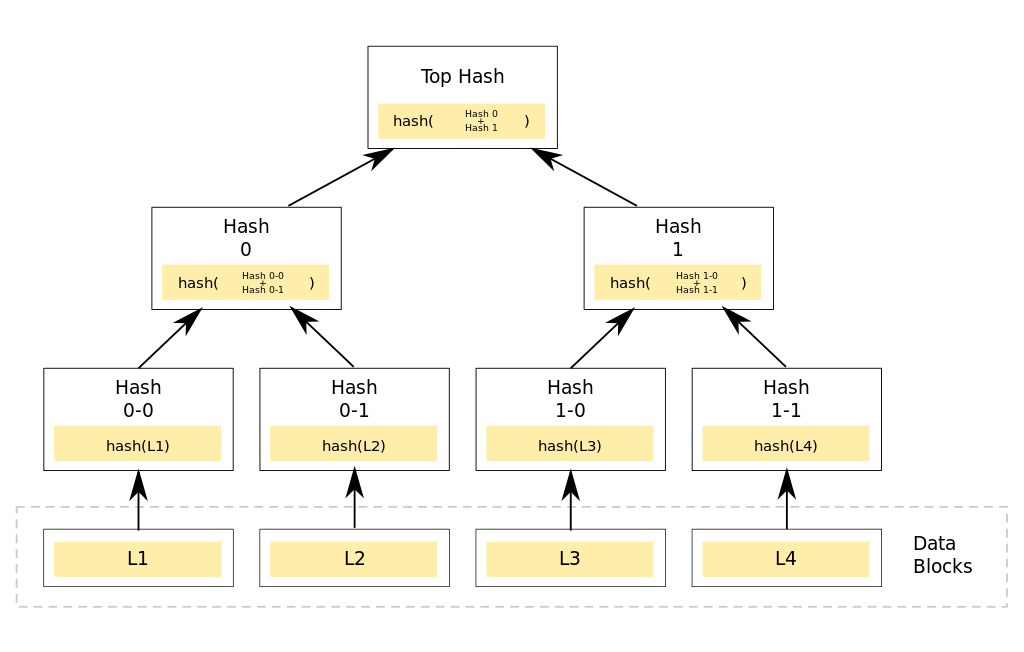
\includegraphics[width=1\textwidth]{immagini/hash_Trees.png}
\caption{Struttura di un merkle tree}
\label{fig:mesh3}

\end{figure}

La figura 2.3 rappresenta un albero di hash binario che può essere generalizzato per visualizzare il procedimento di hashing di un numero arbitrario di transazioni (limitate nella definizione del blocco). Nell'esempio a partire dal basso (o a livello di cardinalità più alto, nelle foglie) si trova contenuto l'insieme delle singole transazioni (L1-L4).

Il primo passo, consiste nell’eseguire l'algoritmo di hashing sulle singole transazioni. L'output di queste operazioni viene successivamente accoppiato con il risultato dell'elemento (nodo) adiacente e su di essi viene di nuovo eseguito l'algoritmo di hashing. Il procedimento è ripetuto ricorsivamente fino a giungere alla radice, risultato di continue applicazioni di hashing nell'insieme di nodi, i quali si trovano a sinistra e destra rispetto alla radice. Dunque, ogni nodo è l'hash dei suoi due figli\footfullcite{ethWhitepaper}. 

Una delle proprietà delle funzioni crittografiche di hash (come SHA-2) consiste, dal punto di vista computazionale di essere veloce da calcolare su qualunque tipo di dato. Inoltre, la peculiarità di questa struttura è che appendere nuove foglie, equivalenti a nuove transazioni che vengono man mano aggiunte all’albero, non comporta la ricomputazione dell’intera struttura ma solo del percorso che porta direttamente alla radice.

Il vantaggio dal punto di vista dell'efficienza dei merkle trees deriva proprio da questa impostazione della struttura gerarchica definita dagli elementi sottostanti. Si tratta dell'efficienza in termini di tempo e dello spazio necessario per memorizzare la struttura. La finalità di Merkle Tree deriva dalla frammentazione dei dati al suo interno e la loro composizione nella radice, sotto un unico identificatore hash. In questo modo per assicurare l'integrità del blocco sarà sufficiente per un nodo verificare la radice della struttura (tx root). Questo è possibile perché la propagazione con la messa insieme di funzioni hash avviene sequenzialmente dalle foglie alla radice.

A livello della blockchain questo apre diverse possibilità di verifica dell'integrità delle singole transazioni e la possibilità di ridurre lo spazio e il tempo necessario per sincronizzare la catena dei blocchi aggiornata all'ultima versione valida. Ad esempio, per un membro della rete che non intende effettuare operazioni su singole transazioni dei blocchi passati sarà sufficiente verificare solo gli hash contenuti nell'intestazione (header) dei blocchi. Se la sincronizzazione, il ricalcolo delle funzioni hash avviene con successo, questo implica l'appartenenza a una catena valida.

\section{Il sistema di consenso} %  Inizio sezione 2.1

Una volta definito il funzionamento concettuale di una rete blockchain. Sorge il dubbio come questo proliferare di operazioni, di calcolo delle funzioni hash, dell'addizione dei nuovi blocchi alla catena e più in generale l'insieme delle operazioni di gestione dell'intera struttura sia possibile in un ecosistema decentralizzato. 

Innanzitutto, le blockchain decentralizzate operano in maniera incentivizzata. La disintermediazione è garantita dagli algoritmi di consenso che stabiliscono le regole di funzionamento della rete. Nel caso delle blockchain pubbliche, si tratta di una rete dove tutti i partecipanti sono alla pari, possono proporre nuove transazioni e tutti insieme devono mettersi d'accordo su quali transazioni effettivamente aggiungere al registro comune. Si vede delineato qui un contesto in cui è presente un insieme di partecipanti ciascuno avente i propri interessi ma nonostante obiettivi spesso contrapposti l'intero sistema deve giungere a un consenso. Tipicamente, l'incentivizzazione consiste in una ricompensa, una quantità di valuta o token, spettante al nodo o ai nodi a cui viene dato il potere di appendere un blocco alla catena. L’approfondimento di questo aspetto economico è strettamente legato al tipo di algoritmo di consenso implementato, alcuni dei quali (ad esempio, Proof of Work e Proof of Stake), verranno discussi più avanti in questa sezione.

\subsection{Il problema dei generali bizantini}

Dal punto di vista teorico, la difficoltà di consenso può essere ricondotta al problema dei generali bizantini\footfullcite{byzantine-generals-problem}. Si suppone che un città venga assediata da molti eserciti con a capo un generale. Per ottenere la vittoria tutti gli eserciti devono raggiungere un consenso e attaccare simultaneamente altrimenti se non attaccano in numero sufficiente verranno sconfitti. La seconda possibilità consiste nella ricezione dell'ordine di ritirata quindi di nuovo un consenso in cui tutti gli eserciti si ritirano unanimemente. Il generale può mandare l'ordine di attaccare oppure di ritirata a tutti gli n-1 comandanti degli eserciti. I comandanti possono mentire scegliendo arbitrariamente di passare ordini diversi e tradire il generale e gli altri comandanti. 

Theorem: For any m, Algorithm OM(m) reaches consensus if there are more than 3m generals and at most m traitors.
This implies that the algorithm can reach consensus as long as 2/3 of the actors are honest. If the traitors are more than 1/3, consensus is not reached, the armies do not coordinate their attack and the enemy wins.

%Si vede delineata qui, ciascuno avente i propri interessi ma nonostante obiettivi spesso %contrapposti l'intero sistema deve giungere a un consenso. In particolare si tratta di %una rete dove tutti i partecipanti possono proporre nuove transazioni e tutti insieme %devono mettersi d'accordo su quali transazioni effettivamente aggiungere al registro %comune.

Un sistema BFT (Byzantine Fault Tolerance) è un sistema che riesce a rimediare al problema dei generali bizantini in un ecosistema decentralizzato. (https://medium.com/loom-network/understanding-blockchain-fundamentals-part-1-byzantine-fault-tolerance-245f46fe8419). Nel caso particolare di Bitcoin e, al momento dello scrivere, Ethereum, si utilizza un protocollo di consenso chiamato Proof of Work che riesce a dare la soluzione al problema sopra esposto.
%Come accennato nel paragrafo 2.1.1 relativo alla questione di distribuzione e decentralizzazione, in un sistema decentralizzato di questo genere 

\subsection{Proof of Work}

Il protocollo Proof of Work, cronologicamente, è il primo sistema di consenso usato nelle blockchain. Implementato per la prima volta da Bitcoin con lo scopo di raggiungere un consenso tra in nodi presenti sulla rete circa lo stato dell’intero sistema. La sua finalità consiste nella gestione e aggiornamento della catena dei blocchi con i relativi elementi in modo che i tutti i partecipanti siano “in linea” con la versione della catena valida cioè la sequenza dei blocchi più lunga. Il legame tra i blocchi una volta validato dal protocollo comporta la creazione di una struttura dei contenuti immutabile contente tutta la storia delle operazioni intercorse fin dalla creazione del blocco genesi.

Senza un punto centrale di calcolo, il procedimento di validazione è incentivizzato per permettere il funzionamento affidabile e costante in un sistema decentralizzato. Nel caso di Proof Of Work, i membri del sistema possono partecipare a una competizione con lo scopo di appendere un blocco alla catena ricevendo in cambio una ricompensa. In questo caso si tratta di dimostrare di aver compiuto una quantità di calcoli computazionali per mezzo di cosiddetti “puzzle crittografici”. Queste dimostrazioni possono ad esempio sfruttare la caratteristica delle funzioni crittografiche di hash per cui il calcolo di una funzione hash comporta la generazione di un risultato
-- DA FARE
distribuito nell’insieme dei risultati possibili.
Ad esempio SHA-2 256bit con 2 alla 256 risultati, 
se nonce = primi 16 bit
+ previene DDOS/SPAM

\subsection{Proof of Stake}

\blindtext

\subsection{Altri Sistemi di Consenso} % Fine sezione 2.1

\section{Funzionamento dell'ecosistema blockchain} % Inizio sezione 2.2

Lorem ute irure dolor in reprehenderit in voluptate velit esse cillum dolore eu fugiat nulla pariatur. Excepteur sint occaecat cupidatat non proident, sunt in culpa qui officia deserunt mollit anim id est laborum.

\subsection{Transazioni e prevenzione della doppia spesa}


Digital signatures, double spend

\subsection{Teoria dei giochi e governabilità}

hardforks

\subsection{Trilemma scalability}

\blindtext

\section{Tipologie di un sistema distribuito} %  Inizio sezione 2.2

Unpermissioned ledgers, Permissioned ledgers, A shared ledger

\subsection{Unpermissioned Ledgers}

\subsection{Permissioned Ledgers}

\blindtext

% direi che non è necessario
%\section{Esempi di applicazione}

%\subsection{Case study 1: Santander money transfer}

%\subsection{Case study 2: Blockchain università di Pisa}

%\subsection{Case study 3: ?}
%\footfullcite{Haber91howto}
%\footfullcite{Kurose:2012:CNT:2584507}
